\chapter{Work Completed}
	\section{Data Accumulation}
		We used dataset created during a Deepfake Image Detection and Reconstruction
		Challenge. Two datasets of real face images were used: CelebA and FFHQ. Various
		Deepfake images were generated using architectures such as StarGAN, GDWCT,
		AttGAN, StyleGAN, and StyleGAN2. Specifically, CelebA images were manipulated
		using pre-trained models available on GitHub for StarGAN, GDWCT, and AttGAN.
		Images from StyleGAN and StyleGAN2 created through FFHQ were obtained. A sample of real and fake images are shown below:

	\begin{figure}[hbt!]
		\centering
		\begin{minipage}{0.45\textwidth}
				\centering
				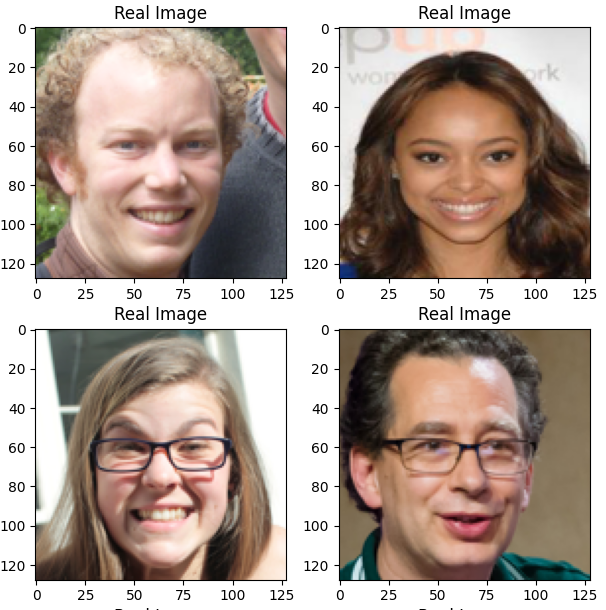
\includegraphics[width=0.95\linewidth]{./img/real sample.png}
				\caption{Real Images}
		\end{minipage}
		\hfill
		\begin{minipage}{0.45\textwidth}
				\centering
				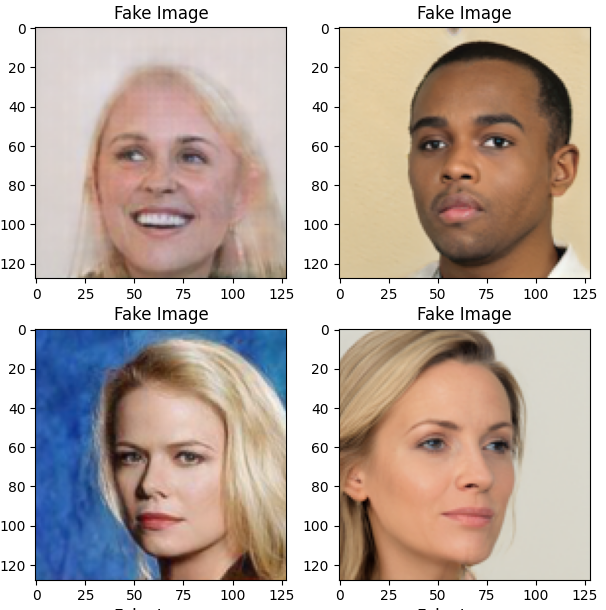
\includegraphics[width=0.95\linewidth]{./img/fake sample.png}
				\caption{Fake Images}
		\end{minipage}
	\end{figure}

	\section{Data Preprocessing}
	\subsection{Data Augmentation}
		To balance our dataset, we augmented our images to achieve a total of 25000 images for each category. For the 5000 fake images, we applied four different transformations, resulting in 20000 augmented fake images. For the real images, we randomly selected and transformed 3750 images, generating 15000 augmented real images. Various transformations, such as rotation, compression, scaling, and mirroring, were implemented. A sample of each transformation is shown below:

	\begin{figure}[hbt!]
		\centering
		\begin{minipage}{0.45\textwidth}
				\centering
				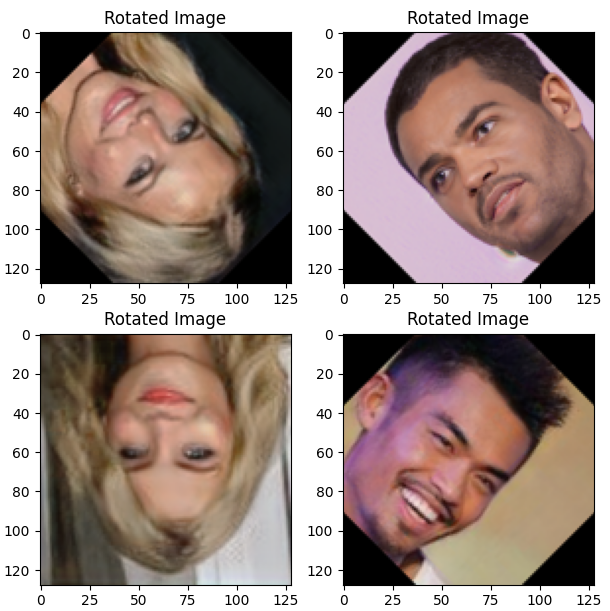
\includegraphics[width=0.95\linewidth]{./img/rotated.png}
				\caption{Rotated Images}
		\end{minipage}
		\hfill
		\begin{minipage}{0.45\textwidth}
				\centering
				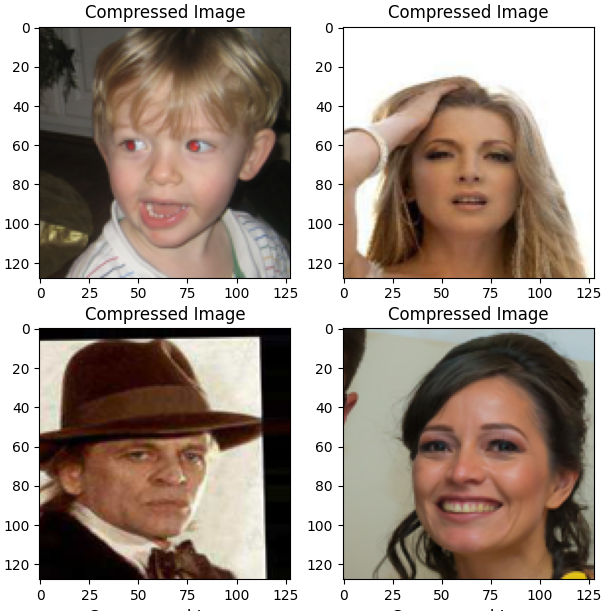
\includegraphics[width=0.95\linewidth]{./img/compressed.png}
				\caption{Compressed Images}
		\end{minipage}

		\vspace{0.5cm} % Add some vertical space between the two rows of images

		\begin{minipage}{0.45\textwidth}
				\centering
				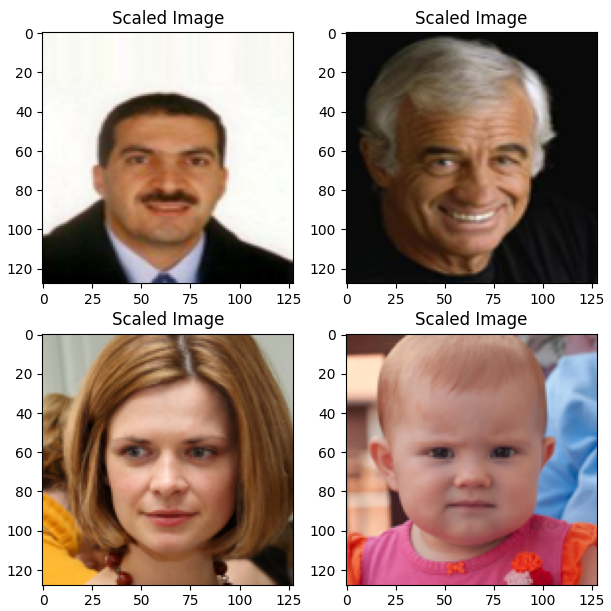
\includegraphics[width=0.95\linewidth]{./img/scaled.png}
				\caption{Scaled Image}
		\end{minipage}
		\hfill
		\begin{minipage}{0.45\textwidth}
				\centering
				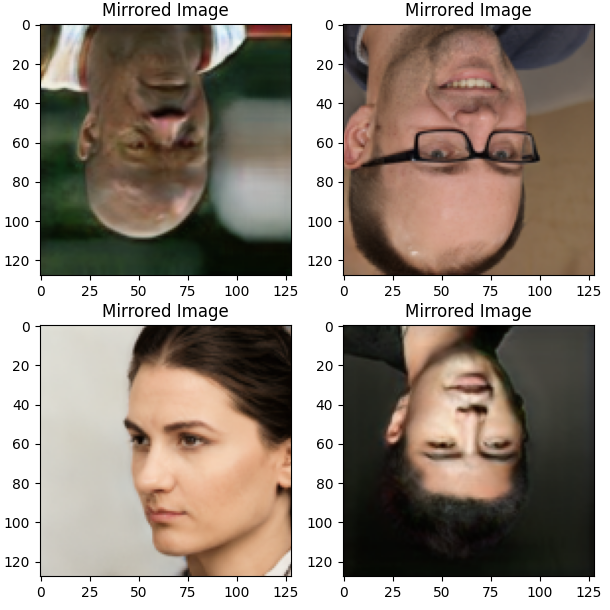
\includegraphics[width=0.95\linewidth]{./img/mirrored.png}
				\caption{Mirrored Images}
		\end{minipage}
	\end{figure}

	\subsection{Data Normalization}
	